\chapter{Graphical Models}

\section{Basics}

\section{Variational Inference}

\subsection{Inference as Optimization: Deriving the ELBO}

Consider a model, $p(\mathbf{x}, \mathbf{z})$, that specifies a joint distribution over a latent variable $\mathbf{z}$ and observed variable $\mathbf{x}$. To infer the posterior distribution of $\mathbf{z}$ given $\mathbf{x}$, we can use the definition of conditional probability:

\begin{equation}
	p (\mathbf{z} | \mathbf{x}) = \frac{p(\mathbf{x}, \mathbf{z})}{p (\mathbf{x})},
	\label{eq: bayes rule}
\end{equation}

\noindent where the marginal likelihood (a.k.a. model evidence or partition function) $p(\mathbf{x})$ is calculated by marginalizing over the latent state space:

\begin{equation}
	p (\mathbf{x}) = \int p(\mathbf{x}, \mathbf{z}) d\mathbf{z}.
	\label{eq: marginalize}
\end{equation}

 \noindent For large latent spaces and/or complicated models, performing the integration in eq. \ref{eq: marginalize} is computationally intractable.
 
 Variational inference transforms this intractable integration problem into an \textit{optimization} problem by introducing an approximate posterior distribution, $q (\mathbf{z} | \mathbf{x})$, typically chosen from some simple family of distributions, such as independent Gaussians. We attempt to make $q (\mathbf{z} | \mathbf{x})$ as ``close" as possible to $p (\mathbf{z} | \mathbf{x})$ by minimizing $ D_{KL}(q (\mathbf{z} | \mathbf{x}) || p (\mathbf{z} | \mathbf{x}))$. Notice that the word close is in quotations because KL divergence is not a true distance measure; it is not symmetric. When the (non-negative) KL divergence between these distributions is zero, we recover the true posterior, $p (\mathbf{z} | \mathbf{x})$. We cannot evaluate $ D_{KL}(q (\mathbf{z} | \mathbf{x}) || p (\mathbf{z} | \mathbf{x}))$ directly, as it includes the true posterior, which we cannot tractably compute. Instead, we will maximize a lower bound on $p(\mathbf{x})$, which will have the effect of minimizing $ D_{KL}(q (\mathbf{z} | \mathbf{x}) || p (\mathbf{z} | \mathbf{x}))$, which we will now show. We start from the definition of KL divergence:
 
 \begin{equation}
 	D_{KL}(q (\mathbf{z} | \mathbf{x}) || p (\mathbf{z} | \mathbf{x})) = \mathbb{E}_{\mathbf{z} \sim q (\mathbf{z} | \mathbf{x})} \left[ \log \frac{q (\mathbf{z} | \mathbf{x})}{p (\mathbf{z} | \mathbf{x})} \right],
	\label{eq: elbo derivation 1}
 \end{equation}
 
 
 \begin{equation}
 	D_{KL}(q (\mathbf{z} | \mathbf{x}) || p (\mathbf{z} | \mathbf{x})) = \mathbb{E}_{\mathbf{z} \sim q (\mathbf{z} | \mathbf{x})} \left[ \log q (\mathbf{z} | \mathbf{x}) \right] - \mathbb{E}_{\mathbf{z} \sim q (\mathbf{z} | \mathbf{x})} \left[ \log p (\mathbf{z} | \mathbf{x}) \right].
	\label{eq: elbo derivation 2}
 \end{equation}
 
 \noindent Plugging in the definition of conditional probability into the second term yields:
 
  \begin{equation}
 	D_{KL}(q (\mathbf{z} | \mathbf{x}) || p (\mathbf{z} | \mathbf{x})) = \mathbb{E}_{\mathbf{z} \sim q (\mathbf{z} | \mathbf{x})} \left[ \log q (\mathbf{z} | \mathbf{x}) \right] - \mathbb{E}_{\mathbf{z} \sim q (\mathbf{z} | \mathbf{x})} \left[ \log \frac{p (\mathbf{x}, \mathbf{z})}{p (\mathbf{x})} \right],
	\label{eq: elbo derivation 3}
 \end{equation}
 
 \noindent which can be expanded into
 \begin{equation}
 	D_{KL}(q (\mathbf{z} | \mathbf{x}) || p (\mathbf{z} | \mathbf{x})) = \mathbb{E}_{\mathbf{z} \sim q (\mathbf{z} | \mathbf{x})} \left[ \log q (\mathbf{z} | \mathbf{x}) \right] - \mathbb{E}_{\mathbf{z} \sim q (\mathbf{z} | \mathbf{x})} \left[ \log p (\mathbf{x}, \mathbf{z}) \right] + \log p (\mathbf{x}).
	\label{eq: elbo derivation 4}
 \end{equation}
 
 \noindent Now, we'll define the following quantity, which we refer to as the \textit{evidence lower bound (ELBO)} or \textit{variational lower bound} or \textit{negative free energy}:
 
\begin{equation}
 	\boxed{\mathcal{L} \triangleq \mathbb{E}_{\mathbf{z} \sim q (\mathbf{z} | \mathbf{x})} \left[ \log p (\mathbf{x}, \mathbf{z}) - \log q (\mathbf{z} | \mathbf{x}) \right]}
	\label{eq: elbo derivation 5}
\end{equation}

\noindent Plugging this definition back into eq. \ref{eq: elbo derivation 4}, we get

   \begin{equation}
 	D_{KL}(q (\mathbf{z} | \mathbf{x}) || p (\mathbf{z} | \mathbf{x})) = \log p (\mathbf{x})  - \mathcal{L}.
	\label{eq: elbo derivation 6}
 \end{equation}
 
 \noindent Rearranging terms, we see
 
    \begin{equation}
 	\log p (\mathbf{x})  =  \mathcal{L} + D_{KL}(q (\mathbf{z} | \mathbf{x}) || p (\mathbf{z} | \mathbf{x})).
	\label{eq: elbo derivation 7}
 \end{equation}

\noindent Since $D_{KL}(q (\mathbf{z} | \mathbf{x}) || p (\mathbf{z} | \mathbf{x}))$ is non-negative, $\mathcal{L}$ is a lower bound on $\log p (\mathbf{x})$. Further, since $\log p (\mathbf{x})$ is not dependent on $q (\mathbf{z} | \mathbf{x})$, we see that maximizing $\mathcal{L}$ with respect to $q (\mathbf{z} | \mathbf{x})$ must minimize $D_{KL}(q (\mathbf{z} | \mathbf{x}) || p (\mathbf{z} | \mathbf{x}))$. Thus, we can approximate the true posterior by optimizing $\mathcal{L}$ with respect to $q (\mathbf{z} | \mathbf{x})$.

Note that the ELBO can also be written in the following form:

\begin{equation}
 	\mathcal{L} = \mathbb{E}_{\mathbf{z} \sim q (\mathbf{z} | \mathbf{x})} \left[ \log p (\mathbf{x}, \mathbf{z}) - \log q (\mathbf{z} | \mathbf{x}) \right]
	\label{eq: elbo derivation 8}
 \end{equation}
 
\begin{equation}
 	\mathcal{L} = \mathbb{E}_{\mathbf{z} \sim q (\mathbf{z} | \mathbf{x})} \left[ \log p (\mathbf{x} | \mathbf{z})  + \log p(\mathbf{z}) - \log q (\mathbf{z} | \mathbf{x}) \right]
	\label{eq: elbo derivation 9}
 \end{equation}
 
\begin{equation}
 	\mathcal{L} = \mathbb{E}_{\mathbf{z} \sim q (\mathbf{z} | \mathbf{x})} \left[ \log p (\mathbf{x} | \mathbf{z}) \right] - D_{KL}(q (\mathbf{z} | \mathbf{x}) || p (\mathbf{z}))
	\label{eq: elbo derivation 10}
 \end{equation}

\noindent This highlights that the ELBO specifies the optimal $q (\mathbf{z} | \mathbf{x})$ by trading off between representing the input, through the first term, and agreeing with the prior on the latent variables, through the second term. In other words, the first term attempts to fit the data, while the second term regularizes the representation.



\subsection{Normalizing Flows} 

A common drawback of variational inference is that it is typically restricted to families of approximate posterior densities, e.g. factorized Gaussians. \textit{Normalizing flows} \cite{rezende2015variational} is a method for fitting flexible approximate posterior densities. It uses a sequence of invertible mappings, called a `flow,' to transform simple posterior densities into arbitrary, flexible forms. If we start with a variable $\mathbf{z}$, drawn from a distribution $q(\mathbf{z})$, and apply an invertible, smooth mapping $f(\mathbf{z})$, then the change of variables formula allows us to write

\begin{equation}
q(\mathbf{z}^\prime) = q(\mathbf{z}) \text{det} \bigg\vert \frac{\partial f^{-1}}{\partial \mathbf{z}^\prime} \bigg\vert = q(\mathbf{z}) \text{det} \bigg\vert \frac{\partial f}{\partial \mathbf{z}} \bigg\vert^{-1}.
\end{equation}
\newline

\begin{figure}[h]
    \centering
    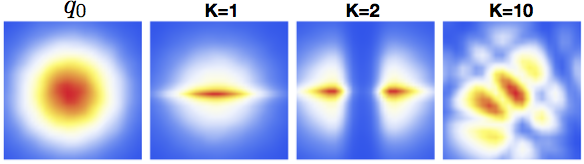
\includegraphics[width=.6\textwidth]{images/graphical_models/normalizing_flows.png}
    \caption{Normalizing flows applied to a 2D isotropic Gaussian, using transformations of the form given in eq. \ref{eq: normalizing flows transformation}. Increasing the flow length $K$ allows for more flexible approximate posterior distributions. Figure reproduced from \cite{rezende2015variational}.}
    \label{fig: full_temporal_model}
\end{figure}

\noindent Note that the mapping, $f$, can also depend on other inputs, such as observed variables $\mathbf{x}$ or other auxiliary inputs. By composing multiple mappings, we can construct arbitrarily complex densities. Thus, starting from an initial distribution of $q_0 (\mathbf{z}_0)$, a flow of length $K$ can be computed as

\begin{equation}
	\log q_K (\mathbf{z}_K) = \log q_0 (\mathbf{z}_0) - \sum_{k=1}^K \log \text{det}  \bigg\vert \frac{\partial f_k}{\partial \mathbf{z}_{k-1}} \bigg\vert.
\end{equation}

\noindent This sequence can be interpreted as performing expansions and contractions on the initial density to construct a more flexible form. 

To parameterize the mappings, \cite{rezende2015variational} use transformations of the form

\begin{equation}
	f(\mathbf{z}) = \mathbf{z} + \mathbf{u}h(\mathbf{w}^\intercal \mathbf{z} + b)
	\label{eq: normalizing flows transformation}
\end{equation}

\noindent where $\mathbf{u}$, $\mathbf{w}$, and $b$ are learned parameters and $h(\cdot)$ is a non-linear function. This class of normalizing flows is referred to as $planar flows$. The determinant of the Jacobian of this transformation is

\begin{equation}
	\text{det} \bigg\vert  \frac{\partial f}{\partial \mathbf{z}} \bigg\vert = \big\vert \text{det} \left( \mathbf{I} + \mathbf{u} (h^\prime (\mathbf{w}^\intercal \mathbf{z} + b) \mathbf{w})^\intercal \right) \big\vert = \big\vert 1 + \mathbf{u}^\intercal h^\prime (\mathbf{w}^\intercal \mathbf{z} + b) \mathbf{w} \big\vert
\end{equation}

\noindent Finally, putting everything together, we can use normalizing flows to draw samples from the final, more flexible approximate posterior, $q(\mathbf{z} | \mathbf{x}) = q_K (\mathbf{z}_K)$. The variational lower bound becomes

\begin{equation}
	\mathcal{L} = \mathbb{E}_{\mathbf{z} \sim q(\mathbf{z}, \mathbf{x})} \left[ \log p(\mathbf{x}, \mathbf{z}) - \log q(\mathbf{z}|\mathbf{x}) \right]
	\label{eq: norm flows lower bound 1}
\end{equation}

\begin{equation}
	\mathcal{L} = \mathbb{E}_{\mathbf{z}_0 \sim q(\mathbf{z}_0, \mathbf{x})} \left[ \log p(\mathbf{x}, \mathbf{z}_K) - \log q(\mathbf{z}_0|\mathbf{x}) + \sum_{k=1}^K \log \big\vert 1 + \mathbf{u}_k^\intercal h_k^\prime (\mathbf{w}_k^\intercal \mathbf{z}_{k-1} + b_k) \mathbf{w}_k \big\vert \right]
	\label{eq: norm flows lower bound 2}
\end{equation}

\noindent Note that in going to eq. \ref{eq: norm flows lower bound 1} to eq. \ref{eq: norm flows lower bound 2} we have used the \textit{law of the unconscious statistician (LOTUS)}, which allows one to take expectations of a transformed variable (or any function thereof) using the original variable. If $\mathbf{z}^\prime = f(\mathbf{z})$ and $g$ is some arbitrary function of $\mathbf{z}^\prime$, then this can be expressed as

\begin{equation}
	\mathbb{E}_{\mathbf{z}^\prime \sim q (\mathbf{z}^\prime)} \left[ g(\mathbf{z}^\prime) \right] = \mathbb{E}_{\mathbf{z} \sim q (\mathbf{z})} \left[ g( f (\mathbf{z})) \right].
\end{equation}

\noindent Thus, we can take expectations with respect to the final density, i.e. the approximate posterior, using samples drawn from the initial density. In an amortized inference setting, the inference model can output the parameters of the initial distribution as well as parameters for each stage of the flow. The flow parameters could also be learned as global parameters.


Another class of normalizing flows is \textit{inverse auto-regressive flow (IAF)} \cite{kingma2016improved}. These transformations take inspiration from auto-regressive models, which factor joint probability distributions into a series of conditional distributions using the chain rule of probability.



\section{Latent Variable Models}

\subsection{Temporal Latent Variable Models}

We have a sequence of observations $\mathbf{x}_{\leq T}$, which extend over $T$ time-steps. Assume we also have a sequence of latent variables $\mathbf{z}_{\leq T}$. If we assume that time only moves in the forward direction, then with parameters $\theta$, we can write the joint probability of this model as

\begin{equation}
	p_\theta (\mathbf{x}_{\leq T}, \mathbf{z}_{\leq T}) = \prod_{t=1}^T p_\theta (\mathbf{x}_{t} | \mathbf{x}_{< t}, \mathbf{z}_{\leq t}) p_\theta (\mathbf{z}_{t} | \mathbf{x}_{< t}, \mathbf{z}_{< t}).
\end{equation}

\noindent The term $p_\theta (\mathbf{x}_{t} | \mathbf{x}_{< t}, \mathbf{z}_{\leq t})$ is the conditional likelihood or observation model, and the term $p_\theta (\mathbf{z}_{t} | \mathbf{x}_{< t}, \mathbf{z}_{< t})$ is the prior, transition, or dynamics model. The full graphical model is represented in figure \ref{fig: full_temporal_model}. The conditional dependencies show that the computation in this model grows exponentially with the sequence length $T$. Later, we will enforce stricter assumptions on the temporal dependencies to make computation tractable.

\begin{figure}[h]
    \centering
    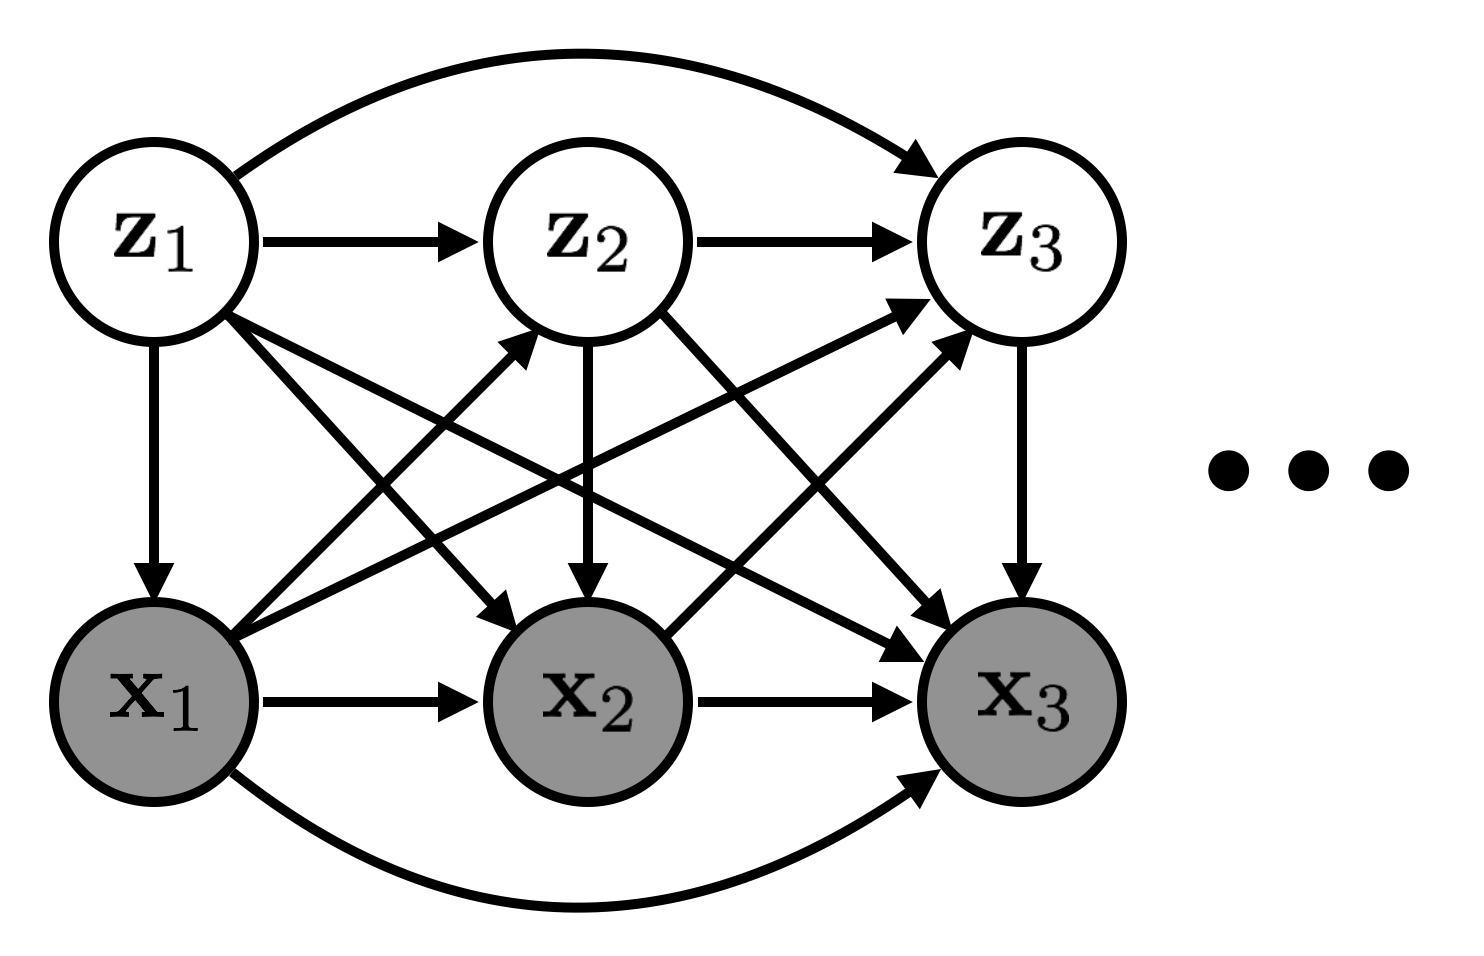
\includegraphics[width=.5\textwidth]{images/graphical_models/full_temporal_model.png}
    \caption{Simplified graphical model representation of temporal latent variable model with all connections present. Note that we're assuming the `arrow of time' points forward; variables can only affect other variables at the current time step or at future time steps. The parameters $\theta$ have been omitted for clarity.}
    \label{fig: full_temporal_model}
\end{figure}

To train or perform inference with this model, we need to compute $p_\theta (\mathbf{x}_{\leq T})$, which involves marginalizing over all states $\mathbf{z}_{\leq T}$:

\begin{equation}
	\log p_\theta (\mathbf{x}_{\leq T}) = \log \int p_\theta (\mathbf{x}_{\leq T}, \mathbf{z}_{\leq T}) d \mathbf{z}_{\leq T}
\end{equation}

\noindent Instead, we'll use an approximate posterior distribution, $q (\mathbf{z}_{\leq T} | \mathbf{x}_{\leq T})$, to compute a lower bound on this quantity:

\begin{equation}
	\log p_\theta (\mathbf{x}_{\leq T}) = \log \mathbb{E}_{q (\mathbf{z}_{\leq T} | \mathbf{x}_{\leq T})} \left[ \frac{p_\theta (\mathbf{x}_{\leq T}, \mathbf{z}_{\leq T})}{q (\mathbf{z}_{\leq T} | \mathbf{x}_{\leq T})} \right]
\end{equation}

\begin{equation}
	\log p_\theta (\mathbf{x}_{\leq T}) \geq \mathbb{E}_{q (\mathbf{z}_{\leq T} | \mathbf{x}_{\leq T})} \left[ p_\theta (\mathbf{x}_{\leq T}, \mathbf{z}_{\leq T}) - q (\mathbf{z}_{\leq T} | \mathbf{x}_{\leq T}) \right]
\end{equation}
